%% module.tex
%
% An Adventure Module class for LaTeX: Example template
%
% Copyright 2016 Michael C. Davis
%
% LICENSE FOR THE WORK
%
% This work consists of the following files:
%    module.cls
%    basic_stats.sty
%    module.tex
%
% This work may be distributed and/or modified under the conditions of the LaTeX
% Project Public License, either version 1.3 of this license or (at your option)
% any later version. The latest version of this license can be found at:
% http://www.latex-project.org/lppl.txt
% and version 1.3 or later is part of all distributions of LaTeX version
% 2005/12/01 or later.
%
% This work has the LPPL maintenance status `author-maintained'.
% 
% The Author and Maintainer of this work is Michael C. Davis
%
%
% LICENSE FOR COMPILED WORKS
%
% You may distribute compiled works generated using the work as specified in
% Clause 3 of the LaTeX Project Public License. If you incorporate Open Gaming
% Content into the compiled work, you must also comply with the terms of that
% license.

%% Start here!
%
% Load the module class. The following options are available:
%
% a4paper         Use A4 paper size (default)
% letterpaper     Use US letter paper size
% sansserif       Use URW Gothic font (similar to ITC Avant Garde Gothic) (default)
% serif           Use ITC Souvenir if available, fall back to URW Bookman if not available
% acdesc          Use descending AC in stat blocks
% acasc           Use ascending AC in stat blocks
% acb1            Use B1-style AC in stat blocks (inspired by http://zenopusarchives.blogspot.com/2014/02/ascending-ac-in-holmes-basic.html)
% acsw            Use Swords & Wizardry style AC in stat blocks
% basic           Use Basic stat blocks (default)
% advanced        Use Advanced stat blocks (not currently implemented, planned for a future release)
%
% In principle, stat blocks can be defined for any RPG system by defining the appropriate style file.
% In this release of the class, only basic_stats.sty is defined.

\documentclass[letterpaper,serif]{module}

% This package generates filler text for the example file, it's not needed in a real project

\usepackage{lipsum}



\begin{document}

%% TITLE PAGE %%
%
% If you want a title page, the minimum requirement is to define author and title, then use \maketitle

\title{Dungeon Module X2$\varepsilon$\\
An Adventure Module Class and Template}

\author{Michael C. Davis}

% The other title page elements are optional

\subtitle{Introductory module for character levels 1--3}

\coverimage{module_art_cover.png}

\abstract{This template is inspired by the old-school modules of the 1980s. It is an attempt to recapture the look and feel
of those classic adventures using the power and beauty of the \LaTeX~typesetting system. The template is designed to allow
authors to typeset their adventures with a minimum of effort. Write your adventure, add some simple markup notation as shown
in the example file, and in a few clicks you will have a beautifully-formatted PDF.}

\copyrightblock{The \LaTeX~module class is Copyright \copyright 2016 Michael Davis and is distributed under the terms
of the \href{http://www.latex-project.org/lppl.txt}{LaTeX Project Public License} (LPPL) Version 1.3c. You are free to use this
class to generate works for distribution, for free or commercially, as detailed in Clause 3 of the license.

Some parts of the template are Copyright \copyright 2000--2003 Wizards of the Coast and are distributed under the
\hyperref[ogl]{Open Game License (OGL)} Version 1.0A.

The images and maps in this example template are not covered by the LPPL. See the license for each work.}

% The contact block is to typeset your logo(s), company name and/or contact details. It consists of three columns; you
% can use any or all of them. By default the columns are top-aligned and of equal width, but you can redefine this in the
% optional argument. See the documentation of the LaTeX tabular environment for details.

\contactblock[p{2.9cm} p{5.0cm} p{9.8cm}]{% column 1 : logo
\begin{center}

\includegraphics[width=1.5cm]{module_logo.pdf}
\end{center}
}{% column 2 : empty in this example
}{% column 3 : contact details
\vspace{0.4cm}
\begin{flushright}
The author can be contacted on Dragonsfoot (user:
\href{http://www.dragonsfoot.org/forums/ucp.php?i=pm&mode=compose&u=7317}{slithy}).\\[0.5em]

Support for the module class and this template will be provided on the
\href{http://www.dragonsfoot.org/forums/viewforum.php?f=87}{Dragonsfoot Computer Gaming \& Utilities} forum.
\end{flushright}
}

% Typeset the title page from the elements above. Remove \maketitle if you don't want a title page.

\maketitle



%% START OF PAGE 1 %%
%
% Display the title text again at the top of the first column.
% Or, use \showtitle[newtext] to use newtext in place of the previously-defined title.

\showtitle

This file is both a short tutorial and example of how to use the module class to typeset your fantasy role-playing game adventure.

\part{Introduction}

The module class is a free resource for authors of adventure modules for fantasy roleplaying games.
It is inspired by the look and feel of the ``Red Book'' Basic incarnation of the world's most popular FRPG.

To prepare your work using this class, you will need \LaTeX, a free document preparation system for high-quality
typesetting. The module class was developed and tested using \TeX Live, which you can download from
\href{https://latex-project.org/ftp.html}{the \LaTeX~Project website}.

Unlike a conventional word processor, the \LaTeX~philosophy is to separate the job of writing and editing content
from the job of typesetting it for publication. Authors can concentrate on writing their text without fussing
about what fonts to choose or what size the page margins or table columns should be. The module class takes care
of all that. Another advantage is that all documents produced using this template will have a similar look and
feel, so if you want to publish a series of works they will appear consistent.

LaTeX uses a markup language in order to describe document structure and presentation. This
file---\verb|module.pdf|---was created from the markup file \verb|module.tex|. If you open \verb|module.tex|
in an ordinary text editor, you will see the markup commands and some explanatory comments (prefixed by \%).
\LaTeX~converts your source text, combined with the markup and the module class, into a high quality PDF document.

You can find numerous tutorials online to get you started with the basics of document preparation using \LaTeX.
The rest of this document is a short tutorial on the module class and examples of its features.

\part{Using the Module Class}

\section{Class Options}

At the beginning of your document, load the module class with \verb|\documentclass[<options>]{module}|. You can
specify the following options:

\begin{description}
\item[a4paper]         Use A4 paper size (default)
\item[letterpaper]     Use US letter paper size
\item[sansserif]       Use a sans-serif font, URW Gothic (default).
\item[serif]           Use a serifed font. This option will use ITC Souvenir if available, URW Bookman otherwise.
\item[acdesc]          Use descending AC in stat blocks (default for Basic stats)
\item[acasc]           Use ascending AC in stat blocks
\item[acb1]            Use \href{http://zenopusarchives.blogspot.com/2014/02/ascending-ac-in-holmes-basic.html}{the B1 AC style} in stat blocks
\item[acsw]            Use \href{http://www.swordsandwizardry.com/}{Swords \& Wizardry} AC style in stat blocks
\item[basic]           Use Basic monster stat blocks (default)
\item[advanced]        Use Advanced monster stat blocks (not currently implemented, planned for a future release)
\end{description}

\subsection*{Paper Size}

The module supports the letter paper size (used in USA) and A4 (used in Europe and the rest of the world). Changing the paper size
does not scale the text on the page; rather it adjusts the margins so the pages will be typeset identically regardless
of which size is selected. This allows module writers to easily create two almost identical PDFs for use in different regions.

As A4 pages are slightly taller, you have the option of a running header if you select \verb|a4paper|.

\subsection*{Fonts}

You can select a serifed or sans-serif font. The default font is URW Gothic (sans-serif), a free font which is similar to
ITC Avant Garde Gothic. Avant Garde was used in many early TSR modules, including B1 and B2.

If you choose the serif option, the module class will check if ITC Souvenir is installed on your system and configured for
\LaTeX~to use. Souvenir is the font used for the 1981 Basic rulebook and several modules of that era. Souvenir is a
commercial font which you must have a license to use. It is expensive to buy the font directly, but it was bundled with some
versions of CorelDraw, so that is a more economical way to obtain a license. To configure the font for use with \LaTeX, you
will need the Adobe Type 1 font definitions (.pfb and .afm files) from CorelDraw and the corresponding LaTeX .tfm and .vf files,
which you can obtain from the \href{https://www.ctan.org/pkg/corelpak}{Corelpak} package. The
\href{https://www.ctan.org/pkg/corelpak-contrib}{Corelpak-contrib} package may also be useful to help with installation.

If you don't have Souvenir installed, the module class will use URW Bookman instead. Bookman is included in the standard
\TeX Live distribution.

\subsection*{Stat Blocks}

This version of the class includes Basic-style monster stat blocks, but it is possible to define a new stat block format for any
RPG system. In principle, authors will be able to compile their work with stats for different systems simply by changing one option
to \verb|documentclass|.

\section{Layout Options}

\subsection*{Headings}

The following heading styles are supported:

\begin{description}
\item[\textbackslash part] Chapter heading (numbered, included in table of contents)
\item[\textbackslash section] Section heading (not numbered, left justified, upper case, included in table of contents)
\item[\textbackslash section*] Section heading (alternate section style, not numbered, centred, included in table of contents)
\item[\textbackslash subsection] Location key (numbered)
\item[\textbackslash subsection*] Other subheading (same style as location key, not numbered)
\item[\textbackslash subsubsection] Sub-location key (numbered with number and letter, e.g. 7a.
\item[\textbackslash subsubsection*] Sub-location key (not numbered, same style as location key)
\end{description}

Location keys are numbered automatically, but you can control the numbering using the \verb|\setcounter| command. For example,
if you want to restart your room location keys at 1 on the second level of your dungeon, just insert |\setcounter{subsection}{0}|
before the first section heading.

If you want a table of contents in your document, simply place a \verb|\tableofcontents| command where you would like it to appear.

\section{Tables}

The module class uses the standard \verb|tabular| environment for tables. You need to specify the horizontal alignment of each column as 
usual. The class provides a \verb|\tableheader| macro which centres the table headings and writes a horizontal rule under each
one. You can redefine the column type for headings: the example below uses the \verb|[b]| option to get bold headings.

\section*{Variable Weapon Damage Table}

\begin{center}
\begin{tabular}{cl}
\tableheader[b]{Damage & Weapon Type}
1-2 (1d2) & Small Fruit Knife\\
1-4 (1d4) & Torch\\
1-6 (1d6) & Hand Axe\\
1-8 (1d8) & Battle Axe\\
1-10 (1d10) & Two-handed sword\\
6-36 (6d6) & Laser Cannon\\
\end{tabular}
\end{center}

\noindent If you need to squeeze wide tables into a text column, you can reduce \verb|\tabcolsep|, which controls the spacing between table columns.

\section*{Character Attacks}

\begin{center}
\addtolength{\tabcolsep}{-4.1pt}
\begin{tabular}{lccccccccccccc}
\tableheader{Attacker's Level & 9 & 8 & 7 & 6 & 5 & 4 & 3 & 2 & 1 & 0 & -1 & -2 & -3}
Normal man & 11 & 12 & 13 & 14 & 15 & 16 & 17 & 18 & 19 & 20 & 20 & 20 & 20\\
1st to 3rd & 10 & 11 & 12 & 13 & 14 & 15 & 16 & 17 & 18 & 19 & 20 & 20 & 20\\
4th + higher & 8 & 9 & 10 & 11 & 12 & 13 & 14 & 15 & 16 & 17 & 18 & 19 & 20\\
\end{tabular}
\addtolength{\tabcolsep}{4.1pt}
\end{center}

\noindent See also: the Wandering Monster table on p.\pageref{wanderingmonsters}.

\section{Monster Stat Blocks}

\monster[Octopodes]{octopus}{Octopus}{7|3*|20'|50'|8|8 legs|1d6 each|Fighter: 10|6|C|1|1-4|X}
\monster{platypus}{Platypus}{7|3*|20'|50'|1|bill|1d4|Fighter: 3|6|C|1|1-4|Y}

First stat block:
\statblock{kobold}{5}{4,4,3,2,1}
Second stat block:
\statblock{kobold}{1}{3}

You must face the \stats[Kobold King!]{kobold}{1}{4}. 
He is with his \stats[10 bodyguards: ]{kobold}{10}{4 each}

\statblock{harpy}{1}{10}
\statblock{harpy}{3}{24 each}

\statblock{octopus}{1}{10}
\statblock{octopus}{3}{24 each}

\statblock{platypus}{1}{10}
\statblock{platypus}{3}{24 each}

\begin{statblockfreestyle}
Jim the Rogue: leather armour, small fruit knife, S7 I12 W5 D17 C12 Ch15. He can backstab with +4 to hit and double damage. AL C
\end{statblockfreestyle}


%%%%% Level One %%%%%

% Float the map on a page on its own

\begin{figure*}[p]
\centering
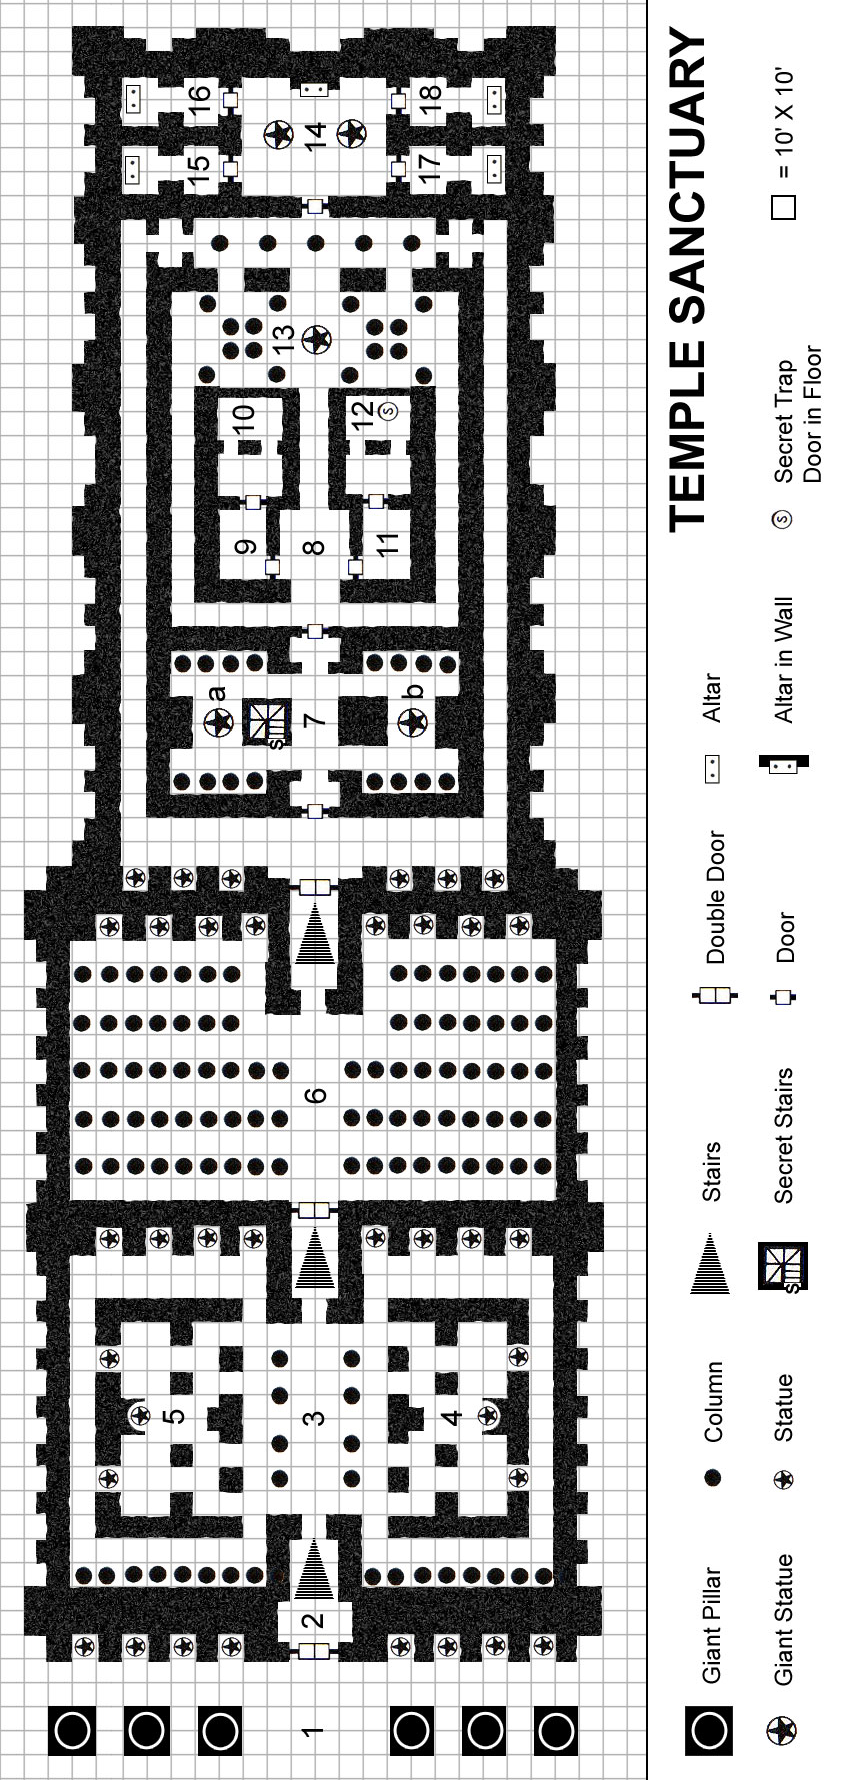
\includegraphics[width=0.75\textwidth]{module_map.png}
\vspace{2em}
\center{Map Copyright \copyright 2008, 2016 Tim Hartin of
\href{http://paratime.ca}{Paratime Design}. Used with permission. All rights reserved.}
\label{img:map}
\end{figure*}

\part{First Dungeon Level}

Some introductory text for the DM.

\section*{Key to Dungeon Level One}

\subsection*{Start}

\begin{boxtext}
Some boxed text to read to the players to introduce them to the adventure.
\end{boxtext}

\subsection{The Portico}                                                        % Key area 1
\label{portico}

Some DM info above the box blah blah blah blah blah blah blah blah blah blah blah blah blah blah blah blah.

% By default, boxed text is moved up by 0.5em to avoid the space below headings (where it is usually placed)
% being too large. If you want to put a box between normal paragraphs, give it the [0pt] parameter to restore
% the default spacing.

\begin{boxtext}[\topsep]
It looks dangerous.
\end{boxtext}

Some monsters are here.
Some DM info below the box blah blah blah blah blah blah blah blah blah blah blah blah blah blah blah blah.

\subsection{Vestibule}                                                          % Key area 2

\begin{boxtext}
blah blah

Multiple paragraphs of boxed text
\end{boxtext}

blah

\subsection{Central Aisle}                                                      % Key area 3

\begin{boxtext}
blah
\end{boxtext}

blah

\vdots                                                                          % Skip areas 4-6

\setcounter{subsection}{7}
\subsubsection{West Court}                                                      % Key area 7a
\label{west_court}

some text

\subsubsection{East Court}                                                      % Key area 7b

some text

\vdots
\setcounter{subsection}{13}                                                     % Skip areas 8-13

\subsection{Inner Sanctuary}                                                    % Key area 14
\label{inner_sanctuary}

more text

\begin{figure}[ht]
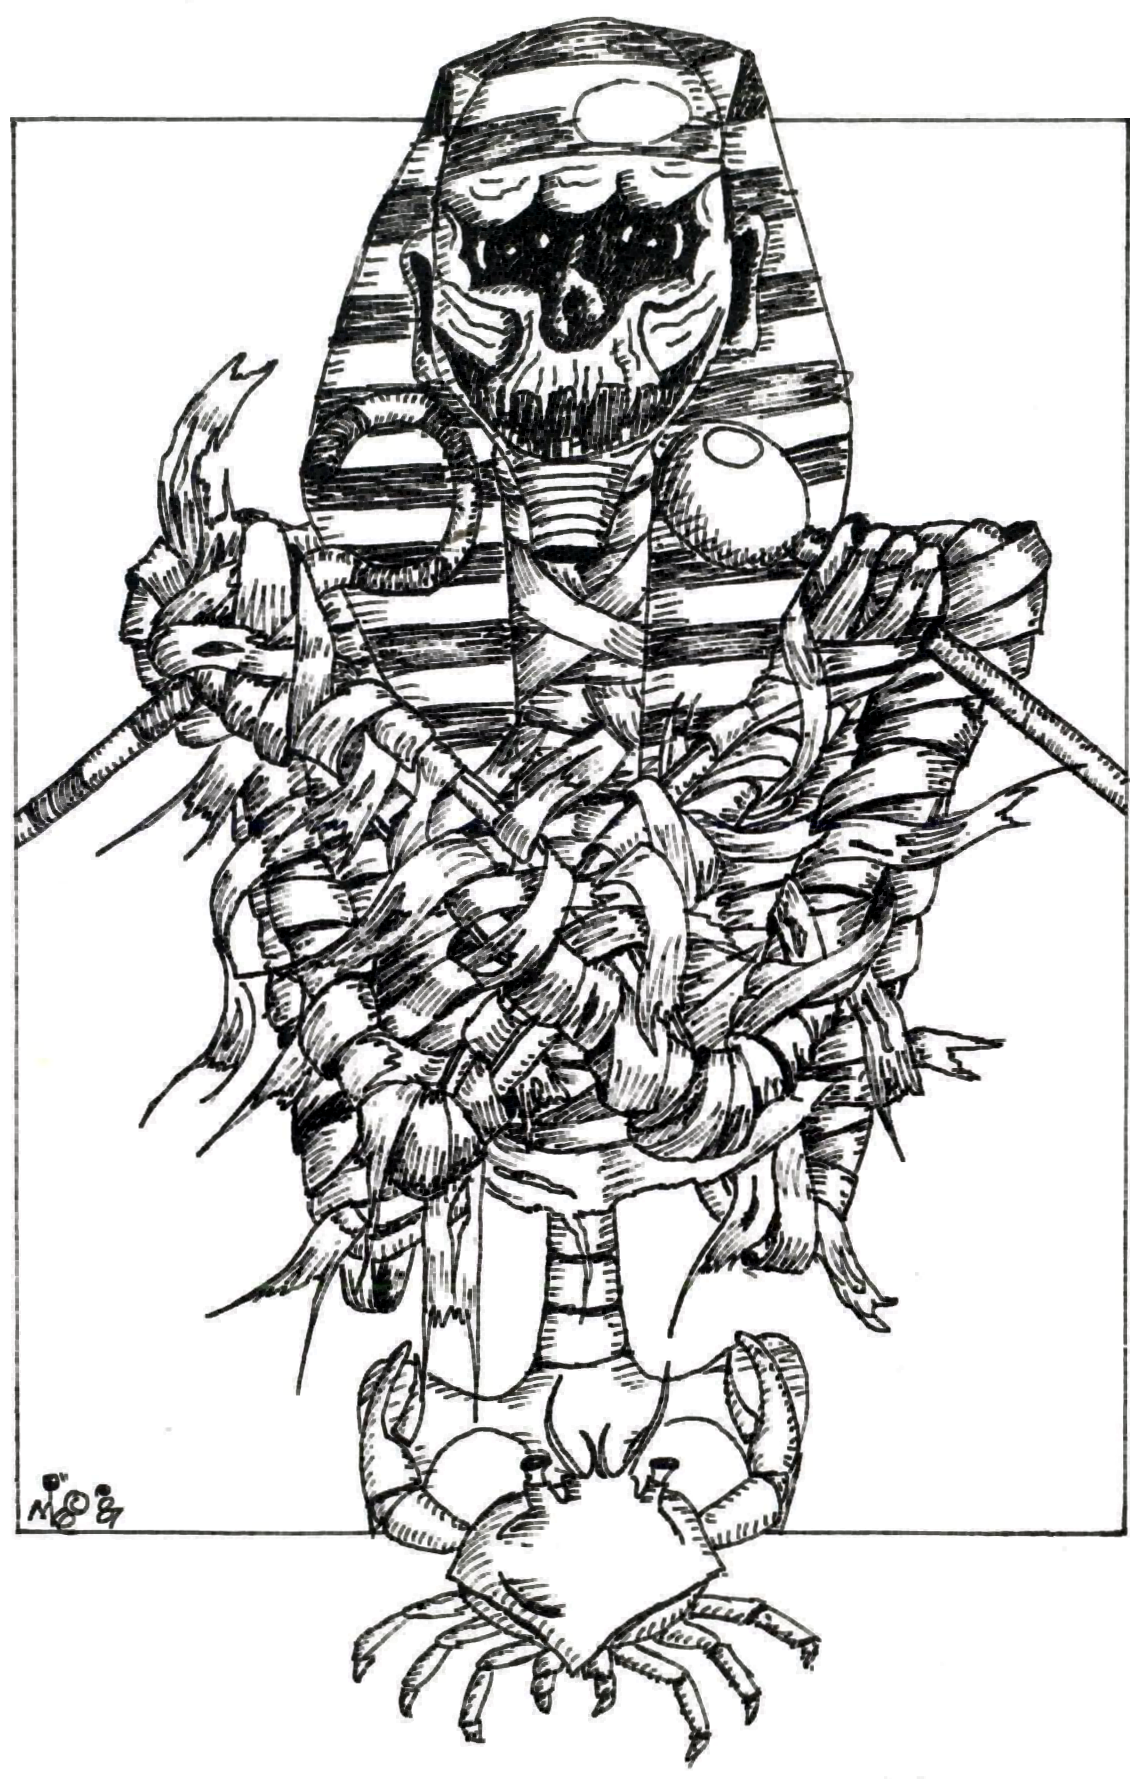
\includegraphics[width=\columnwidth]{module_art_interior.png}
\center{Tomb It May Concern.\\
Image Copyright \copyright 1987, 2016 Michael Davis. All rights reserved.}
\label{img:tomb}
\end{figure}

%%%%% Level Two %%%%%

\begin{onecolumnfloat}[t]
\part{Second Dungeon Level}

If you want to have some pages with a single column of text, you can use \verb|\onecolumn| to switch
into one-column mode and \verb|\twocolumn| to switch back to two-column mode. These commands cause
a page break.

If you want to mix single and double-column text on the same page, use the \verb|onecolumnfloat| environment
to create a float which is the full width of the page. You can do the same thing with graphics using
the \verb|figure*| environment, as we do for the map on p.\pageref{img:map}.

\section*{Wandering Monsters}
\label{wanderingmonsters}

\begin{wanderingmonsters}[b]
\wanderitem{kobold}{3-18}
\wanderitem{kobold}{}
\wanderitem{harpy}{1-4}
\wanderitem[8-10]{octopus}{2}
\wanderitem[11]{octopus}{}
\wanderitem{platypus}{2}
\wanderitem{platypus}{}
\end{wanderingmonsters}

\section*{Monster Roster}

\begin{monsterroster}
\rosteritem{\ref{portico}}{kobold}{16}{4 each}
\rosteritem{\ref{west_court}}{harpy}{1}{23}
\rosteritem{\ref{inner_sanctuary}}{harpy}{3}{18 each}
\end{monsterroster}
\end{onecolumnfloat}

\lipsum

%
% New Monsters part
%

\part{New Monsters}

\begin{newmonster}{kobold}
These small, evil dog-like men\ldots

\lipsum
\end{newmonster}

\begin{newmonster}{octopus}
Octopodes are cunning and evil.
\end{newmonster}

Text following the monster block.

\part{License Information}

The \LaTeX~module class is Copyright \copyright 2016 Michael Davis and is distributed under the terms of the
\href{http://www.latex-project.org/lppl.txt}{LaTeX Project Public License} (LPPL) Version 1.3c.

You are free to use the class to generate works for your own private use and/or for distribution as detailed in
Clause 3 of the license. There is no restriction on commercial use.

An acknowledgement is much appreciated: you can use the \verb|\modulecopyright| macro to insert an acknowledgement
block. No payment is required or expected, but if you wish to express your appreciation you are welcome to do so via
\href{https://paypal.me/slithy}{PayPal}.

%
% License section
%

\section{Open Game Content}
\label{ogl}

The template includes three macros to make it easy to distribute your work under the Open Game License
from Wizards of the Coast: \verb|\ogl|, \verb|\productidentity| and \verb|\opengamecontent|. You can see
an example below:

\begin{ogl}
% This environment includes the complete text of the OGL v1.0A. Within the environment, you should include
% the exact text of the COPYRIGHT NOTICE of any other OGL text you are copying, modifying or distributing.
% Usually this will include the title, copyright date and copyright holder's name(s). Example:
\item System Reference Document, Copyright \copyright 2000--2003, Wizards of the Coast, Inc., by Jonathan Tweet, Monte Cook,
Skip Williams, Rich Baker, Andy Collins, David Noonan, Rich Redman, Bruce R. Cordell, John D. Rateliff, Thomas Reid, James
Wyatt, based on original material by E. Gary Gygax and Dave Arneson.
\end{ogl}

\begin{productidentity}
\item The text of this \LaTeX~module class and example template, which comprises all typesetting elements and all text which
is not explitly Open Game Content, is Product Identity.
\modulecopyright

\item All photographs, artwork and maps in this template are Product Identity.

\item The cover image is adapted from an original image on
\href{https://commons.wikimedia.org/wiki/File:Karnak_Tempel_Vorhof_05.jpg}{Wikimedia Commons}, copyright \copyright 2009 Olaf
Tausch. Used with permission under the terms of the
\href{https://creativecommons.org/licenses/by/3.0/deed.en}{Creative Commons Attribution 3.0 Unported} license.

\item The map on p.\pageref{img:map} is copyright \copyright 2008, 2016 Tim Hartin of \href{http://paratime.ca}{Paratime Design}.
Used with permission. All rights reserved.

\item The drawing on p.\pageref{img:tomb} is copyright \copyright 1987, 2016 Michael Davis. All rights reserved.
\end{productidentity}

\begin{opengamecontent}
\item The monster statistics from the SRD are Open Game Content.
\end{opengamecontent}

%
% Table of Contents
%

\tableofcontents

% If you would also like to include an index for your document, see the LaTeX makeidx package

\end{document}
